\section{Conclusões preliminares: Rumo aos dados observados}\label{Conclusao_Modelo}

Esta pesquisa pretende contribuir para a literatura de crescimento liderado pela demanda do modelo do supermultiplicador sraffiano, levando em consideração o esforço recente de incorporá-lo em um arcabouço contábil do tipo SFC.  A característica específica do modelo aqui apresentado é a inclusão do investimento residencial. A introdução desse gasto tem como objetivo dar conta dos resultados de alguns trabalhos empíricos recentes que mostram a importância do investimento residencial para dinâmica macroeconômica e, como visto anteriormente, nenhum trabalho ainda havia incorporado esse gasto específico. 

O modelo reproduz as principais características do supermultiplicador sraffiano: (i) o grau de utilização converge ao grau normal, por meio de variações da propensão marginal a investir das firmas e; (ii) a taxa de crescimento da economia segue a taxa de crescimento dos gastos autônomos – nesse caso, o investimento residencial. A primeira diferença do  presente modelo é que o estoque de capital fixo da economia passa a ter dois componentes, o capital produtivo das firmas e os imóveis das famílias. 

Como visto nas simulações, o principal resultado particular deste modelo é que uma maior taxa de crescimento do investimento residencial tem como consequência uma redução da participação do estoque de imóveis no capital total. Tal resultado, aparentemente contra intuitivo, se deve ao ajuste do estoque de capital das firmas. Para que o grau efetivo de utilização da capacidade convirja ao grau normal, o investimento das firmas precisa temporariamente crescer mais rápido que investimento residencial, alterando, portanto, a relação entre os dois estoques. 

Os outros dois experimentos trazem resultados em linha com o supermultiplicador sraffiano. O aumento da participação dos salários na renda não afeta a taxa de crescimento de longo prazo e, portanto, não afeta a propensão marginal a investir de forma permanente. Porém, por alterar o tamanho do supermultiplicador, aumenta a participação do capital produtivo no capital total. O aumento da taxa de juros, por sua vez, tem um efeito tanto sobre a taxa de crescimento de longo prazo quanto sobre o endividamento das famílias em relação à renda disponível. 

É importante destacar que este trabalho é apenas o primeiro passo numa agenda de pesquisa mais ampla sobre o papel do investimento residencial no ciclo e no crescimento econômico. Pesquisas futuras podem (e devem) tornar o modelo aqui apresentado mais complexo. Possíveis extensões incluem explorar os determinantes do investimento residencial, para levar em consideração o efeito de bolhas de preços dos imóveis no comportamento da demanda agregada, e acrescentar o consumo de duráveis, que alguns trabalhos empíricos apontam como fortemente influenciados pela dinâmica imobiliária. 

\begin{figure}[H]
	\centering
	\caption{Inserindo Taxa Própria, taxa de juros hipotecária e inflação de móveis observada}
	\label{choque_Real}
	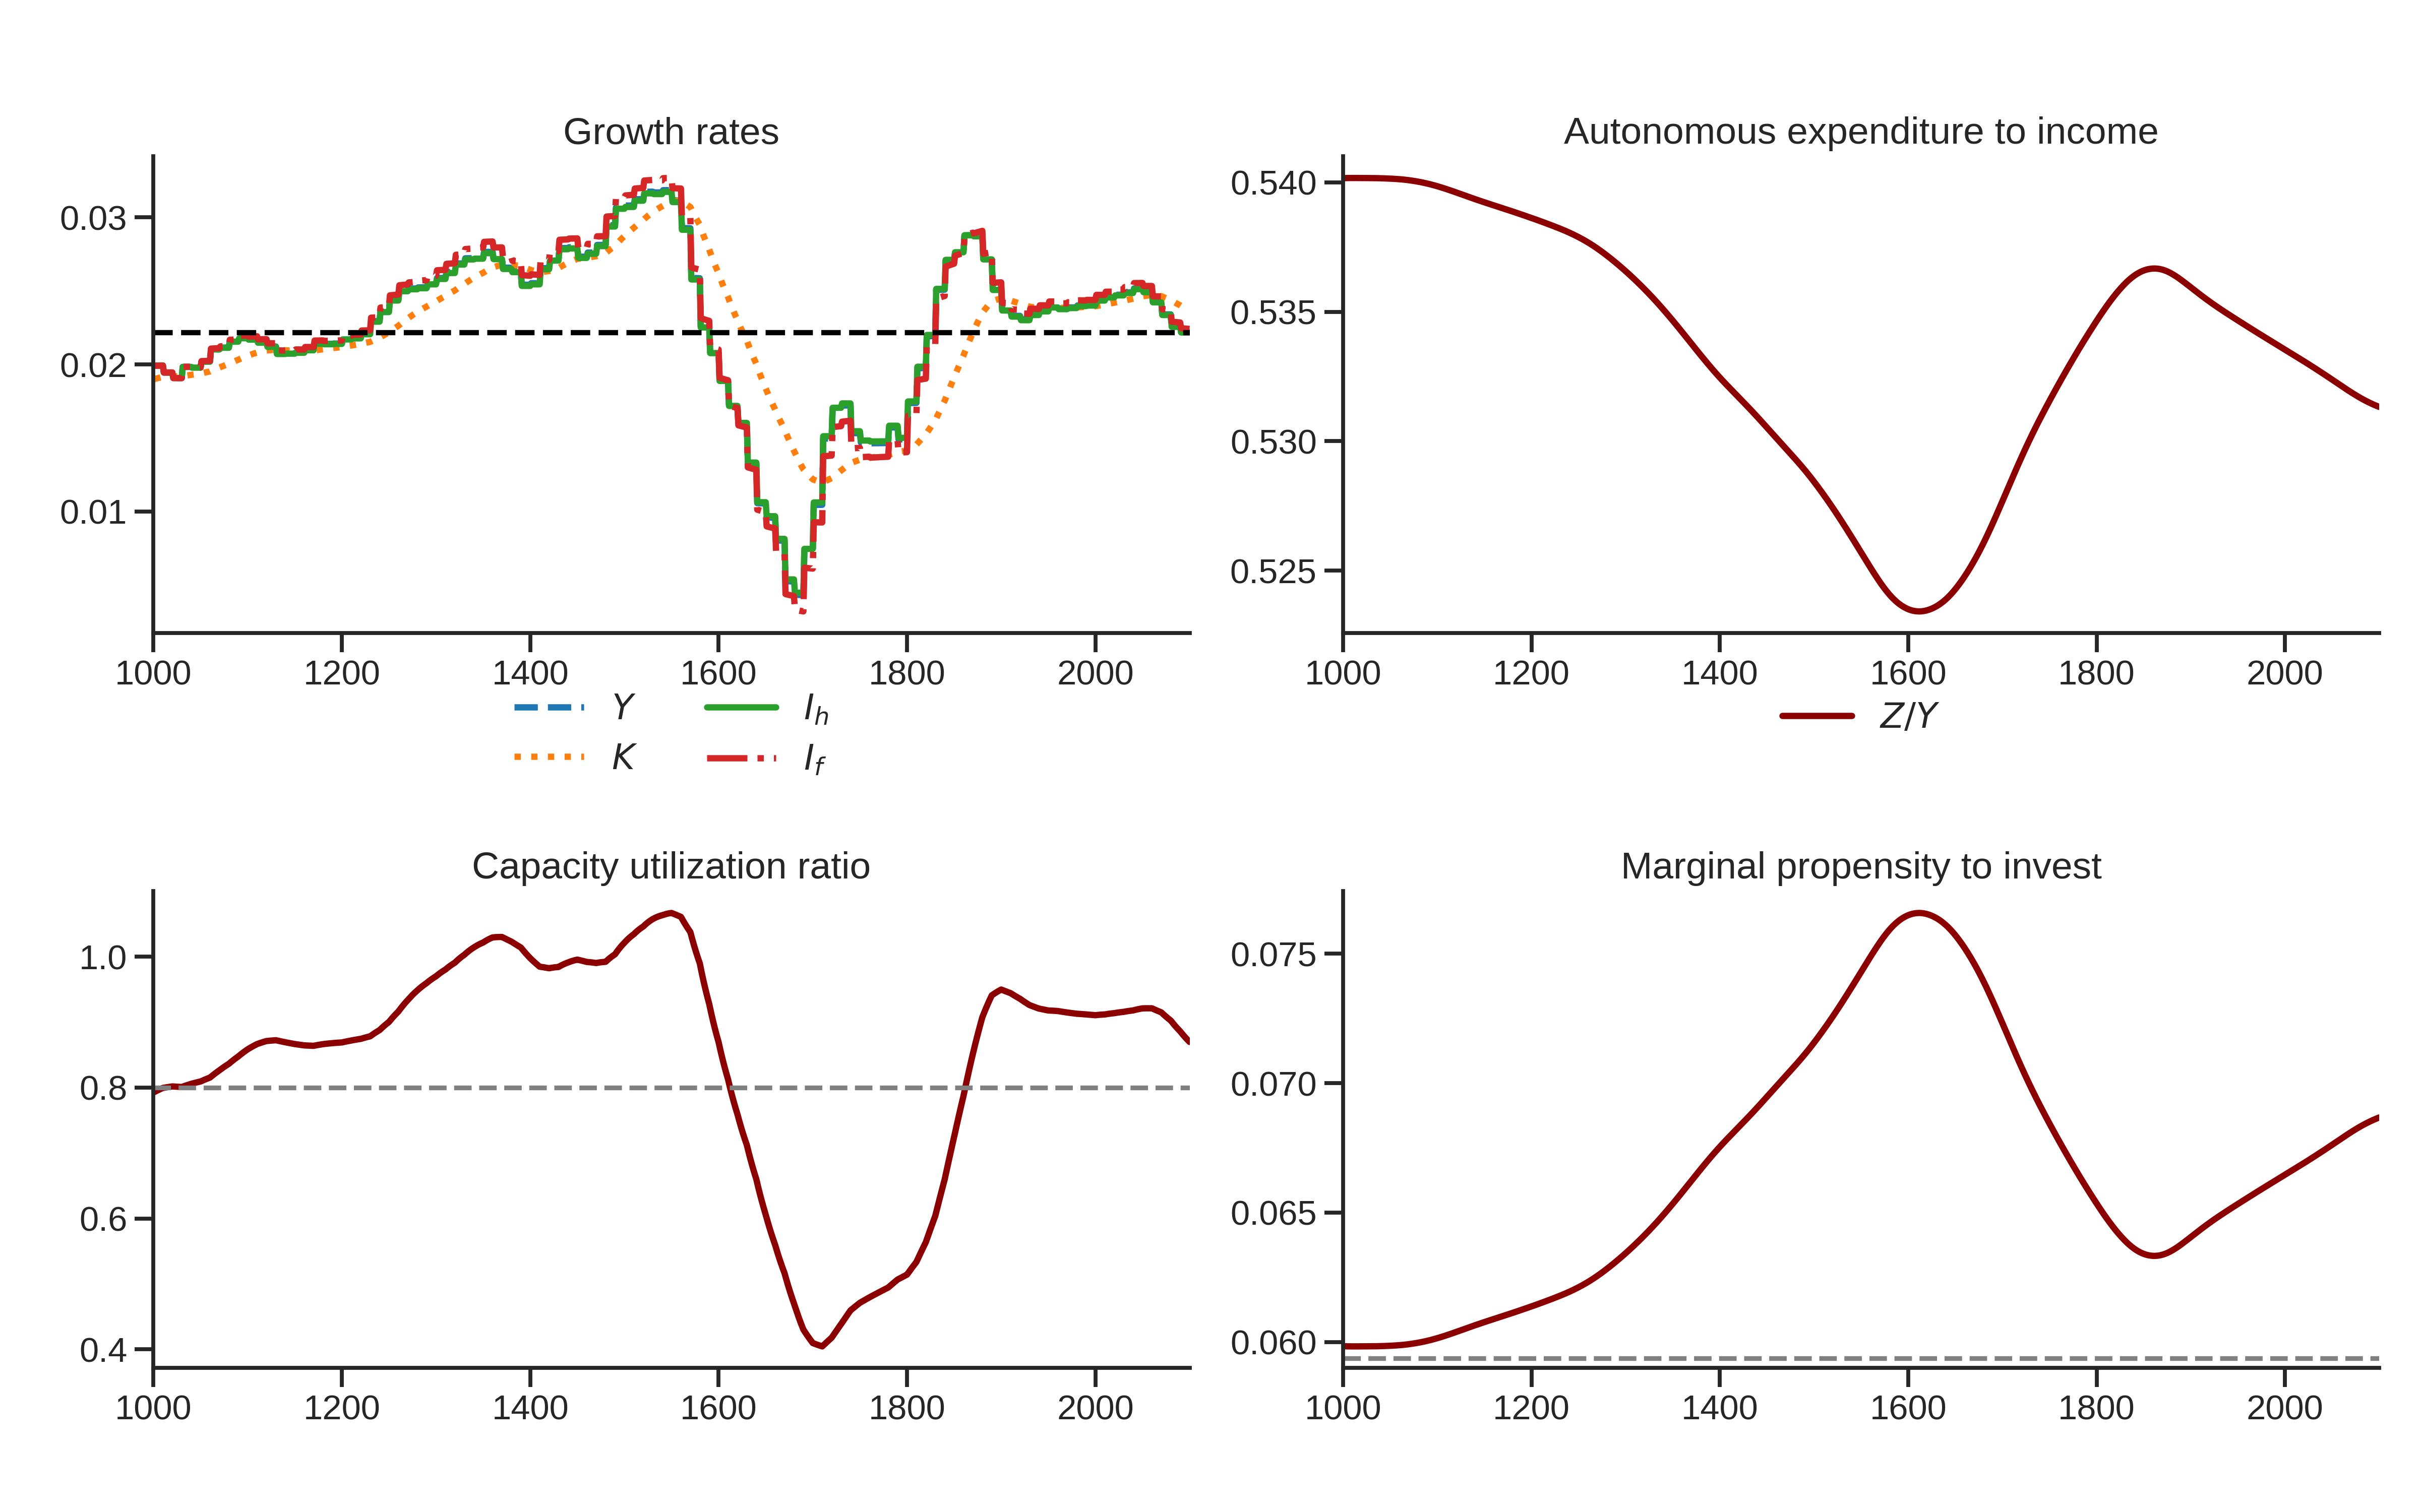
\includegraphics[width=\textwidth]{../../Modelo/Versoes/Shock_Real.png}
	\caption*{\textbf{Fonte:} Elaboração própria}
\end{figure}


\begin{figure}[H]
	\centering
	\caption{Inserindo Taxa Própria, taxa de juros hipotecária e inflação de móveis observada}
	\label{choque_Real}
	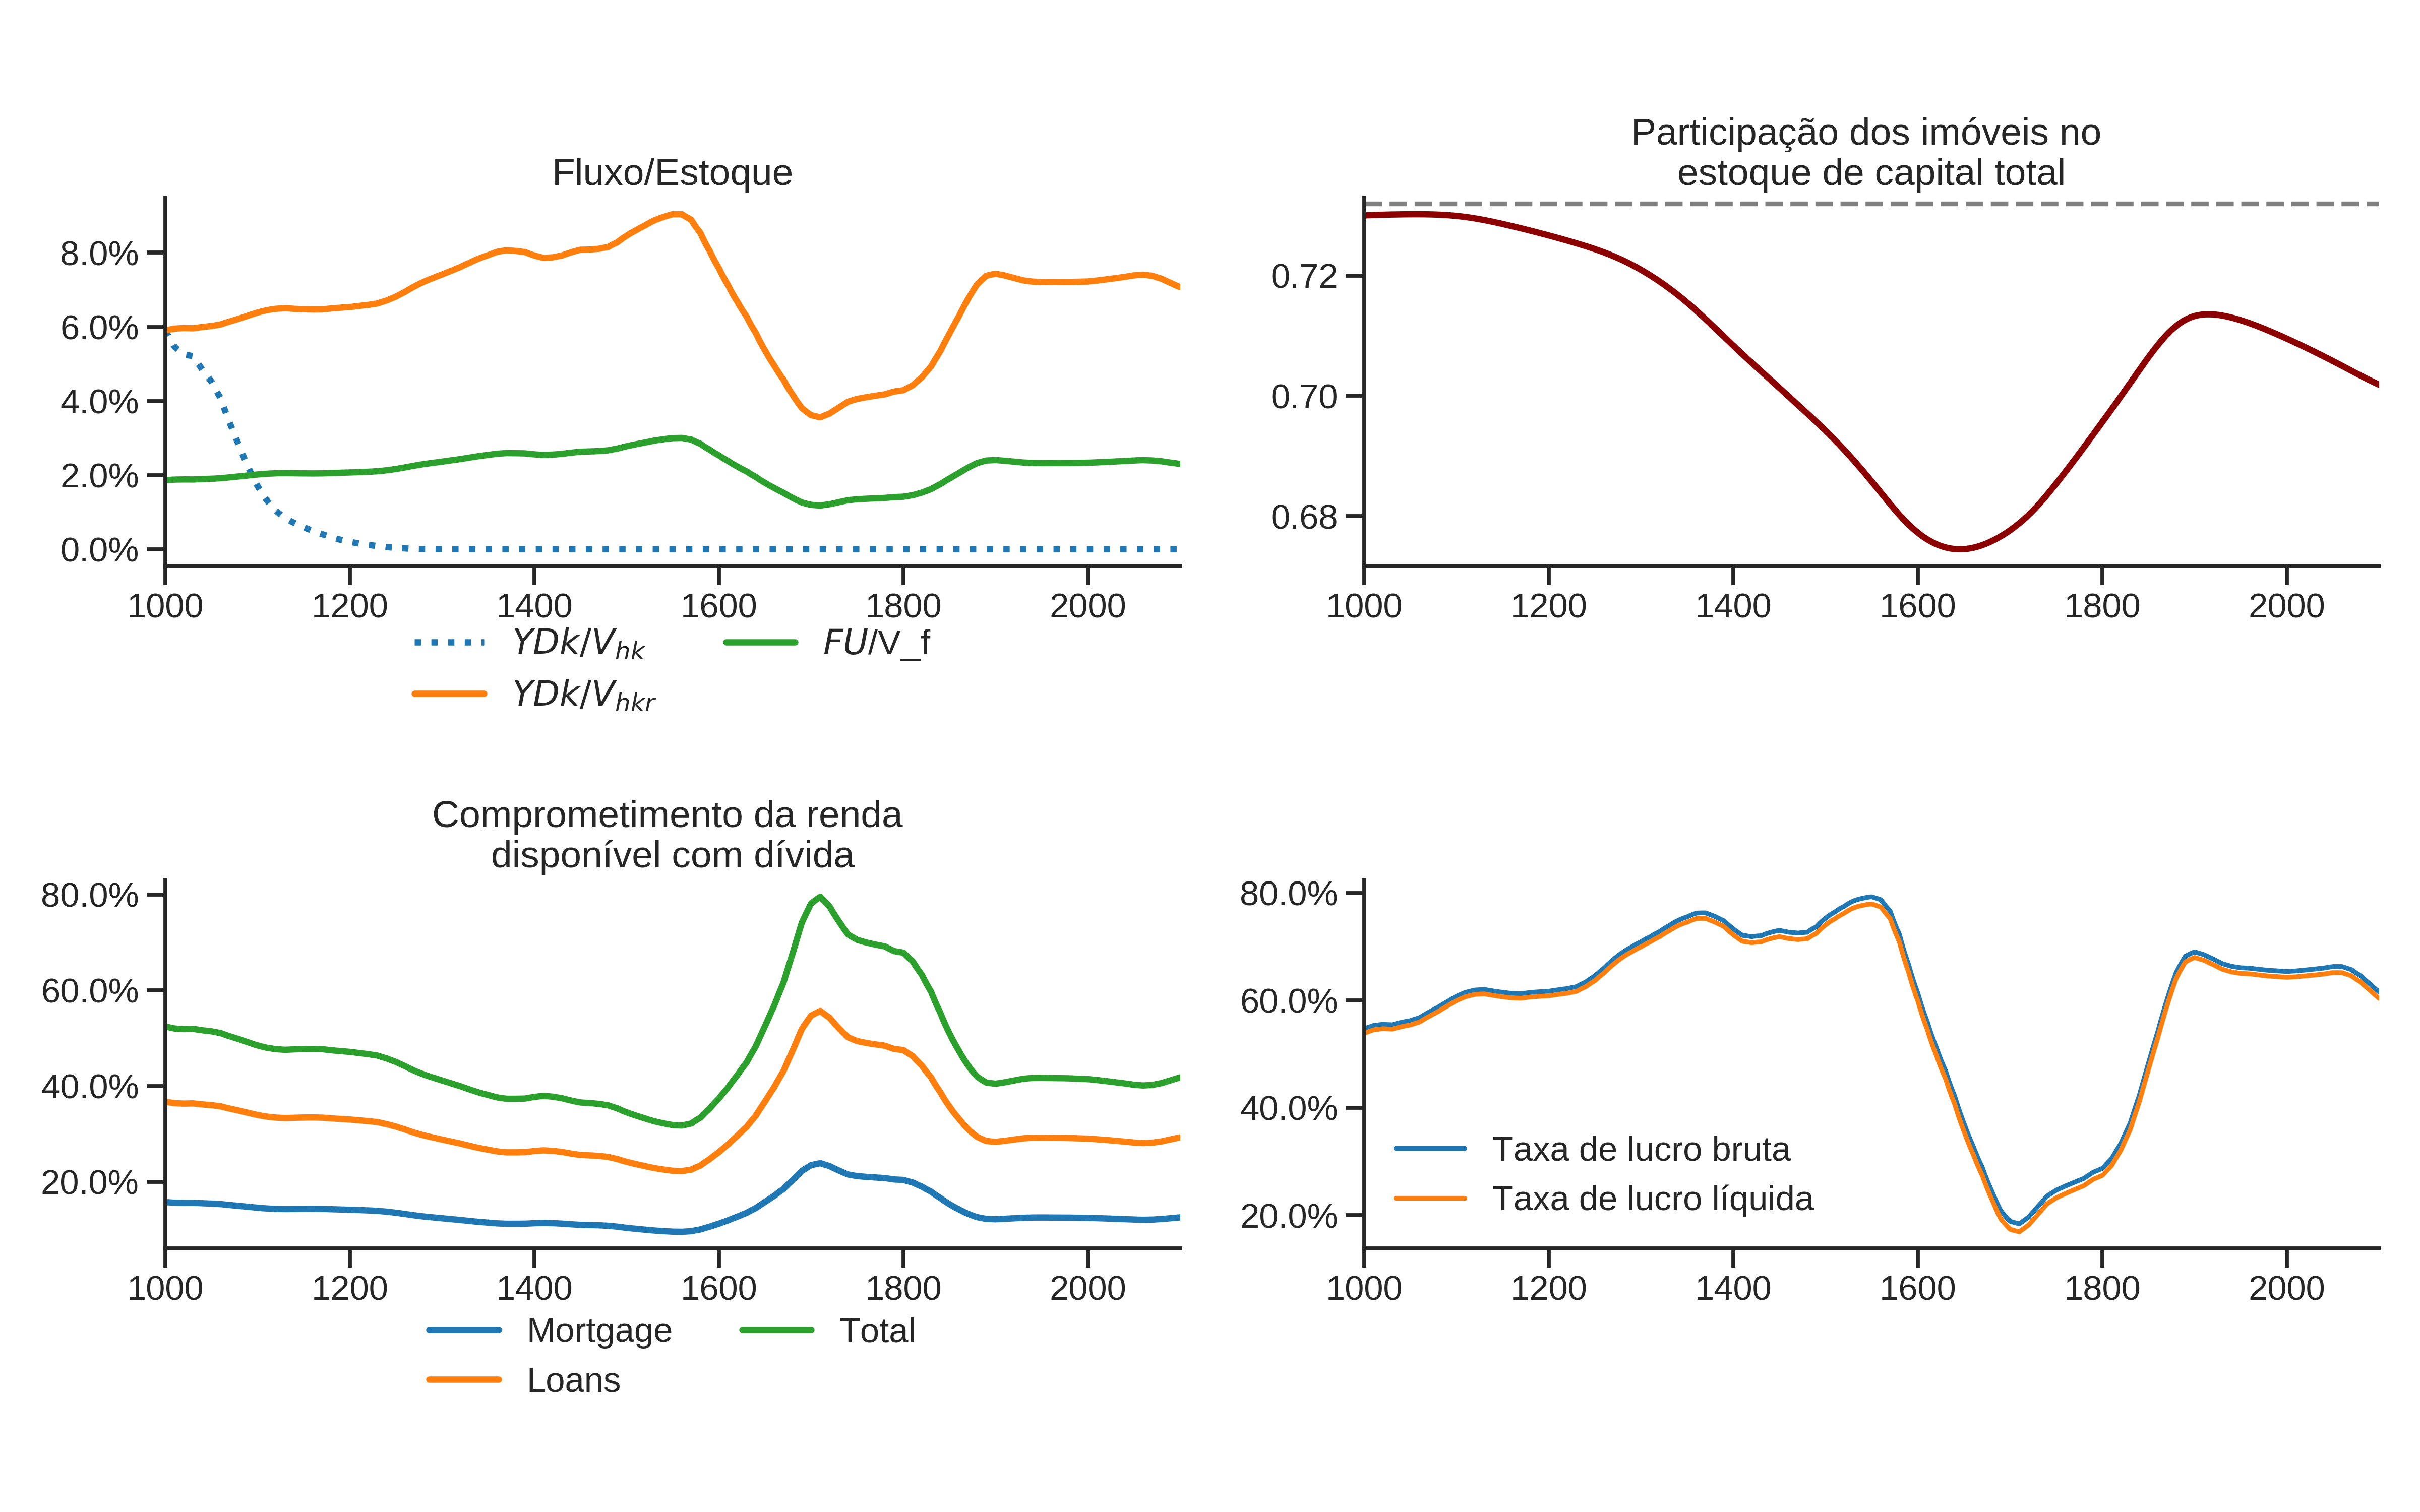
\includegraphics[width=\textwidth]{../../Modelo/Versoes/Shock_RealNorms.png}
	\caption*{\textbf{Fonte:} Elaboração própria}
\end{figure}